
\documentclass{beamer}

\usepackage{algpseudocode, color, colortbl}

\usepackage{wrapfig}

\usetheme{Montpellier}
\usecolortheme{rose}

% page numbers, from
% https://tex.stackexchange.com/questions/137022/how-to-insert-page-number-in-beamer-navigation-symbols
\expandafter\def\expandafter\insertshorttitle\expandafter{%
  \insertshorttitle\hfill%
  \insertframenumber\,/\,\inserttotalframenumber}

\definecolor{Gray}{gray}{0.8}
\newcolumntype{g}{>{\columncolor{Gray}}c}

\newcommand{\stanza}{ \\~\ }

\newcommand{\naive}{na\"{i}ve~}
\newcommand{\Naive}{Na\"{i}ve~}

\title{12. Dynamic Programming for Matrix Chain Multiplication}
\subtitle{CPSC 535}
\author{Kevin A. Wortman}
\institute{ 
\includegraphics[height=2cm]{csuf-logo-cmyk} }
\date{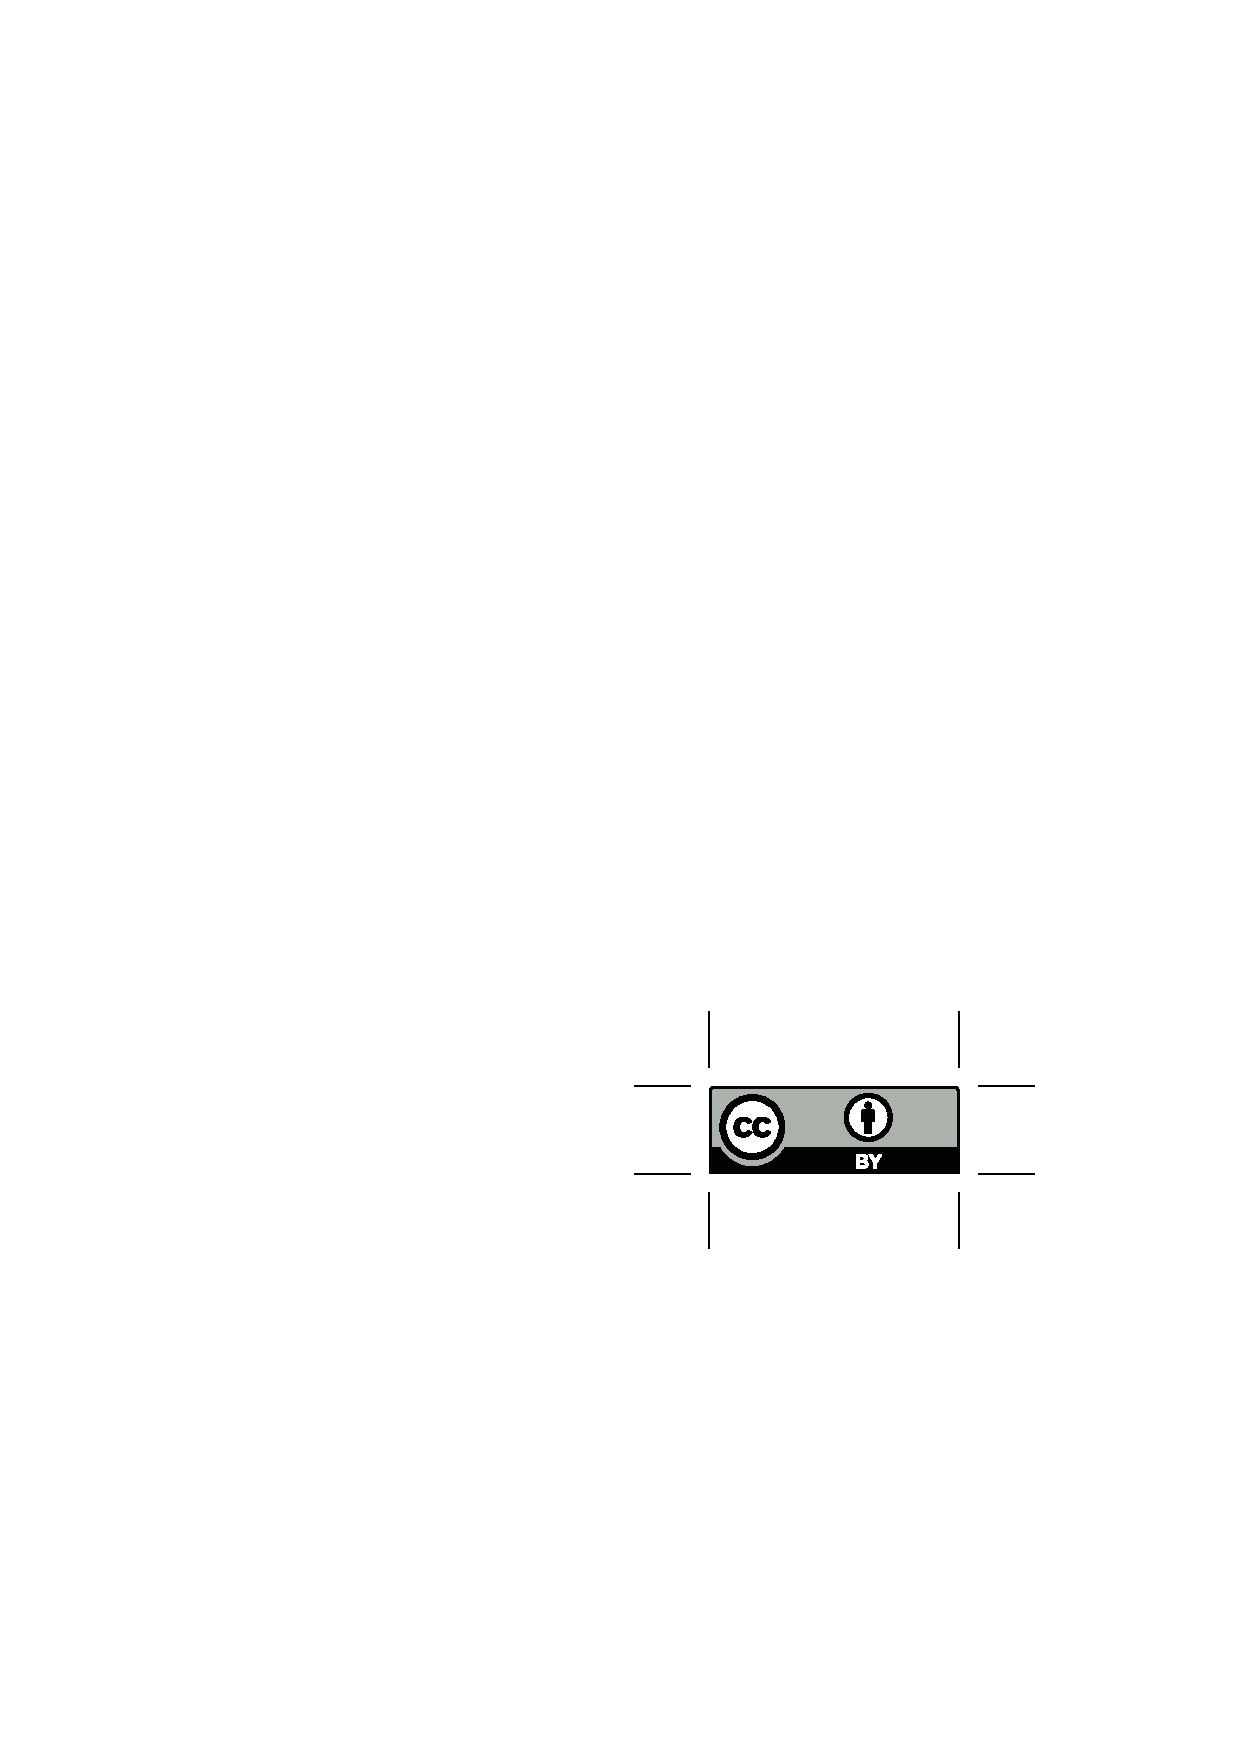
\includegraphics[height=14pt]{by} \\

{\tiny
This work is licensed under a
\href{http://creativecommons.org/licenses/by/4.0/}{Creative Commons Attribution 4.0 International License}.
}}

\begin{document}

\begin{frame}
  \titlepage
\end{frame}

\begin{frame} \frametitle{Big Idea: 2D Table}
\begin{itemize}
  \item \emph{Recall:} dynamic programming
  \begin{itemize}
    \item problem has recursive structure
    \item overlapping subproblems
    \item use table to store solutions, avoid duplicated effort
    \item top-down or bottom-up
  \end{itemize}
  \item so far: \textbf{1D table} -- has one index
  \item now: \textbf{2D table} -- has \emph{two} indices
\end{itemize}
\end{frame}

\begin{frame} \frametitle{Matrix Multiplication}
  for matrices $A_1, A_2:$
  \[ A_1 A_2 \]

  Recall:
  \[
  \begin{bmatrix}
    \textcolor{red}{5} & \textcolor{red}{12} & \textcolor{red}{5} \\
    16 & 9 & 4
  \end{bmatrix}
  \times
  \begin{bmatrix}
    \textcolor{red}{19} & 2 \\
    \textcolor{red}{9} & 5 \\
    \textcolor{red}{8} & 11
  \end{bmatrix}
  =
  \begin{bmatrix}
    \textcolor{red}{5 \times 19 + 12 \times 9 + 5 \times 8} & 125 \\
    417 & 121 
  \end{bmatrix}
  \]
\end{frame}

\begin{frame} \frametitle{Matrix Multiplication Algorithms}
Recall:
  \begin{itemize}
    \item \Naive algorithm: three nested loops, $O(n^3)$
    \item Strassen's algorithm: divide-and-conquer, $\approx O(n^{2.8074})$
    \item Those analyses assumed $A_1, A_2$ are both square $n \times n$ matrices
    \item Now: matrix sizes may differ
    \item \textbf{Compatible:} $A_1$ and $A_2$ are compatible when $A_1.columns = A_2.rows$
  \end{itemize}
\end{frame}

\begin{frame} \frametitle{\Naive Matrix Multiplication Algorithm}
  {\small
  \begin{algorithmic}[1]
    \Function{MATRIX-MULTIPLY}{A, B}
    \State $C = $ new $A.rows \times B.columns$ matrix
    \For { $i$ from 1 to $A.rows$ }
      \For { $j$ from 1 to $B.columns$ }
        \State $c_{ij} = 0$
        \For { $k$ from 1 to $A.columns$ }
          \State $c_{ij} = c_{ij} + a_{ik} \cdot b_{kj}$
        \EndFor
      \EndFor
    \EndFor
    \State \Return $C$
    \EndFunction
  \end{algorithmic}
  }
  
  \textbf{Analysis:} $\Theta(A.rows \times A.columns \times B.columns)$
\end{frame}

\begin{frame} \frametitle{Matrix Chain Multiplication}
  Given $n$ compatible matrices $A_1, A_2, \ldots, A_n,$ compute
  \[ A_1 A_2 \ldots A_n \]

  \begin{itemize}
    \item Recall: matrix multiplication is \textbf{associative}
    \item May parenthesize $ A_1 A_2 \ldots A_n $ in any order
    \item Q: which order is most efficient?
  \end{itemize}
\end{frame}

\begin{frame} \frametitle{Equivalent Parenthesizations}
 \begin{align*}
    A_1 A_2 A_3 A_4
    &= A_1 (A_2(A_3 A_4)) \\
    &= A_1 ((A_2 A_3) A_4) \\
    &= (A_1 A_2) (A_3 A_4) \\
    &= (A_1 (A_2 A_3)) A_4 \\
    &= ((A_1 A_2) A_3) A_4
  \end{align*}
\stanza

\begin{center}
  Total runtime depends on the dimensions of $A_1 \ldots A_4.$
\end{center}
\end{frame}

\begin{frame} \frametitle{Example: Different Runtimes}
Given three matrices $A_1, A_2, A_3$ with dimensions
\begin{center}
  \begin{tabular}{l|ll}
    matrix & rows & columns \\ \hline
    $A_1$ & 10 & 100 \\
    $A_2$ & 100 & 5 \\
    $A_3$ & 5 & 50
  \end{tabular}
\end{center}
\begin{itemize}
  \item $((A_1 A_2)A_3)$ costs $10 \cdot 100 \cdot 5 + 10 \cdot 5 \cdot 50= 5,000+2,500 = 7,500$ scalar multiplies
  \item $(A_1 (A_2 A_3))$ costs $100 \cdot 5 \cdot 50 + 10 \cdot 100 \cdot 50 = 25,000 + 50,000 = 75,000$ scalar multiplies
  \item first is order of magnitude faster
\end{itemize}
\end{frame}

\begin{frame} \frametitle{Matrix Chain Multiplication Problem}
  \emph{matrix chain multiplication problem} \\
  \textbf{input:} a sequence $\langle A_1, A_2, \ldots, A_n \rangle$ of $n>0$ compatible matrices,
    and sequence $p=\langle p_0, p_1, \ldots, p_n \rangle$ of integers, where
    matrix $A_i$ has $p_{i-1}$ rows and $p_i$ columns \\
  \textbf{output:} a parenthesization of $A_1 A_2 \ldots A_n$ that minimizes scalar multiplications
  \stanza

  \emph{matrix chain multiplication value problem} \\
  \textbf{input:} a sequence $\langle A_1, A_2, \ldots, A_n \rangle$ of $n>0$ compatible matrices,
    and sequence $p=\langle p_0, p_1, \ldots, p_n \rangle$ of integers, where
    matrix $A_i$ has $p_{i-1}$ rows and $p_i$ columns \\
  \textbf{output:} the minimum number of scalar multiplies necessary to multiply $A_1 A_2 \ldots A_n$ 
\end{frame}

\begin{frame} \frametitle{Design Process}
  \begin{enumerate}
    \item Identify the problem's \textbf{solution} and \textbf{value}, and note which is our \textbf{goal}.
    \item Derive a \textbf{recurrence} for an optimal value.
    \item Design a divide-and-conquer algorithm that computes an \textbf{optimal value}.
    \item Design a dynamic programming algorithm that computes an \textbf{optimal value}.
    \begin{enumerate}
      \item \textbf{top-down} alternative: add table base case (\textbf{memoization})
      \item \textbf{bottom-up} alternative: rewrite to use bottom-up loops instead of recursion
    \end{enumerate}
    \item (if goal is a solution algo.) Design a dynamic programming algorithm that computes an \textbf{optimal solution}.
  \end{enumerate}
  \end{frame}
  
\begin{frame} \frametitle{Matrix Chain Multiplication Step 1}
\begin{enumerate}
  \item Identify the problem's \textbf{solution} and \textbf{value}, and note which is our \textbf{goal}.
  \stanza
\end{enumerate}
\emph{matrix chain multiplication value problem} \\
\textbf{input:} a sequence $\langle A_1, A_2, \ldots, A_n \rangle$ of $n>0$ compatible matrices,
  and sequence $p=\langle p_0, p_1, \ldots, p_n \rangle$ of integers, where
  matrix $A_i$ has $p_{i-1}$ rows and $p_i$ columns \\
\textbf{output:} the minimum number of scalar multiplies necessary to multiply $A_1 A_2 \ldots A_n$ 
\begin{itemize}
  \item \textbf{solution:} parenthesized expression e.g. $(A_1(A_2 A_3))(A_4 A_5)$
  \item \textbf{value:} number of multiplications e.g. $75,000$
  \item goal: \textbf{value}
\end{itemize}
\end{frame}

\begin{frame} \frametitle{Matrix Chain Multiplication Step 2}
  \begin{enumerate}
    \setcounter{enumi}{1}
    \item Derive a \textbf{recurrence} for an optimal value.
    \stanza
  \end{enumerate}

  \begin{itemize}
    \item define $r_{i, j} = $ minimum number of multiplies for $A_i A_{i+1} \ldots A_j$
    \item (note: \textbf{two} indices)
    \item solution to whole problem is $r_{1, n}$
    \item base case: $A_i$ by itself; so when $i=j,$ $r_{i,\, j} = 0$
    \item general case:
    \begin{itemize}
      \item \textbf{think} divide-and-conquer; define $r_{i, j}$ in terms of $r_{<i, <j}$
      \item make the problem \textbf{one piece} smaller
      \item given $A_i A_{i+1} \ldots A_j$, split w/ parenthesis at index $k:$
        \[ A_i A_{i+1} \ldots A_j = (A_i A_{i+1} \ldots A_k) (A_{k+1} A_{k+2} \ldots A_j) \]
      \item try every option and keep the optimal one
      \[ r_{i, j} = \min_{i \leq k \leq \, j} r_{i, k} + r_{k+1, \, j} + p_{i-1} p_k p_j \]
    \end{itemize}
  \end{itemize}
\end{frame}
  
\begin{frame} \frametitle{Matrix Chain Multiplication Step 3}
  \begin{enumerate}
    \setcounter{enumi}{2}
    \item Design a divide-and-conquer algorithm that computes an \textbf{optimal value}.
    \stanza
  \end{enumerate}

  {\scriptsize
  \begin{algorithmic}[1]
    \Function{MATRIX-CHAIN-VALUE-DC}{$p[0..n]$}
    \State \Return{MC-DC($p, 0, n$)}
    \EndFunction
    \Function{MC-DC}{$p[0..n], i, j$}
    \If{ $i==j$ }
      \State \Return{ 0 }
    \EndIf
    \State $q = \infty$
    \For {$k$ from $i$ to $j-1$}
      \State $q = \min(q, \text{MC-DC}(p, i, k) + \text{MC-DC}(p, k+1, j) + p[i-1] \times p[k] \times p[\, j])$
    \EndFor
    \State \Return{$q$}
    \EndFunction
  \end{algorithmic}
  }
\end{frame}

\begin{frame} \frametitle{Sidebar: Analysis of MATRIX-CHAIN-VALUE-DC}
\begin{itemize}
  \item MC-DC-REC calls itself $O(n)$ times in general case
  \item like CUT-ROD-DC
  \item exponential time
  \item again, dynamic programming will circumvent all this recursion
\end{itemize}
\end{frame}

\begin{frame} \frametitle{Matrix Chain Multiplication Step 4.a}
  \begin{enumerate}
    \setcounter{enumi}{3}
    \item Design a dynamic programming algorithm that computes an \textbf{optimal value}.
    \begin{enumerate}
      \item \textbf{top-down} alternative: add table base case (\textbf{memoization})
      \stanza
    \end{enumerate}
\end{enumerate}

\begin{itemize}
  \item Recall \textbf{memoization:} use a hash dictionary to make a ``memo'' of pre-calculated solutions
  \item create hash table $T$
  \item use pair $(i, j)$ as key in table $T,$ storing $r_{i,\, j}$
\end{itemize}
\end{frame}

\begin{frame} \frametitle{Matrix Chain Multiplication Step 4.a}
  {\scriptsize
  \begin{algorithmic}[1]
    \Function{MATRIX-CHAIN-VALUE-MEMOIZED}{$p[0..n]$}
    \State HASH-TABLE-CREATE($T$)
    \State \Return{MC-M($T, p, 1, n$)}
    \EndFunction
    \Function{MC-M}{$T, p[0..n], i, j$}
    \State $q = $ HASH-TABLE-SEARCH($T, (i, j)$)
    \If{ $q \ne$ NIL }
      \State \Return{ $q$ }
    \EndIf
    \If{ $i==j$ }
      \State $q=0$
    \Else
      \State $q = \infty$
      \For {$k$ from $i$ to $j-1$}
        \State $q = \min(q, \text{MC-M}(p, i, k) + \text{MC-M}(p, k+1, j)+ p[i-1] \times p[k] \times p[\, j])$
      \EndFor
    \EndIf
    \State $q.key = (i, j)$
    \State HASH-TABLE-INSERT($q$)
    \State \Return{$q$}
    \EndFunction
  \end{algorithmic}
  }
\end{frame}

\begin{frame} \frametitle{Memoized Algorithm Analysis}
  \begin{itemize}
    \item $T$ contains $\Theta(n^2)$ pairs $(i, j)$
    \item each entry is inserted exactly once
    \item in the general case, MC-M takes $\Theta(n)$ expected time
    \item $\Rightarrow$ MATRIX-CHAIN-VALUE-MEMOIZED takes $\Theta(n^3)$ expected time
  \end{itemize}
\end{frame}

\begin{frame} \frametitle{Matrix Chain Multiplication Step 4.b}
  \begin{enumerate}
    \setcounter{enumi}{3}
    \item Design a dynamic programming algorithm that computes an \textbf{optimal value}.
    \begin{enumerate}
      \item \textbf{top-down} alternative: add table base case (\textbf{memoization})
      \item \textbf{bottom-up} alternative: rewrite to use bottom-up loops instead of recursion
      \stanza
    \end{enumerate}
\end{enumerate}

\begin{itemize}
  \item create 2D array $m$ where $m[i][\, j] = r_{i, \, j}$
  \item \textbf{bottom-up:} write an explicit \textbf{for} loop that computes and stores every general case
  \item need to order loops so we never use an uninitialized element
  \item $\therefore$ initialize chain length $1 \text{(base case)}, 2, \ldots, n$
\end{itemize}
\end{frame}

\begin{frame} \frametitle{Matrix Chain Multiplication Step 4.b}
  {\footnotesize
  \begin{algorithmic}[1]
    \Function{MATRIX-CHAIN-BU}{p[0..n]}
    \State Create array $m[1..n][1..n]$
    \For{$i$ from 1 to $n$}
      \State $m[i][i] = 0$ \Comment{base case, length=1}
    \EndFor
    \For{$\ell$ from 2 to $n$} \Comment{$\ell$ = general-case length}
      \For{$i$ from $1$ to $(n-\ell+1)$}
        \State $j = i + \ell - 1$
        \State $q=\infty$
        \For{$k$ from $i$ to $j-1$}
          \State $q = \min(q, m[i][k] + m[k+1][\,j] + p[i-1] \times p[k] \times p[\,j])$
        \EndFor
        \State $m[i][\,j] = q$
      \EndFor
    \EndFor
    \State \Return $m[1][n]$
    \EndFunction
  \end{algorithmic}
  }
\end{frame}

\begin{frame} \frametitle{Matrix Chain Multiplication Analysis}
  \begin{itemize}
    \item MATRIX-CHAIN-BU is clearly $\Theta(n^3)$ time
    \item top-down memoized algorithm: $\Theta(n^3)$ expected time
    \item bottom-up algorithm: $\Theta(n^3)$ time with faster constant factors
  \end{itemize}
\end{frame}

\begin{frame} \frametitle{Matrix Chain Multiplication Step 5}
  \begin{enumerate}
    \setcounter{enumi}{4}
    \item (if goal is a solution algo.) Design a dynamic programming algorithm that computes an \textbf{optimal solution}.
    \stanza
  \end{enumerate}

  \emph{matrix chain multiplication value problem} \\
  \textbf{input:} a sequence $\langle A_1, A_2, \ldots, A_n \rangle$ of $n>0$ compatible matrices,
    and sequence $p=\langle p_0, p_1, \ldots, p_n \rangle$ of integers, where
    matrix $A_i$ has $p_{i-1}$ rows and $p_i$ columns \\
  \textbf{output:} the minimum number of scalar multiplies necessary to multiply $A_1 A_2 \ldots A_n$ 
  \stanza

  \emph{matrix chain multiplication problem} \\
  \textbf{input:} (same) \\
  \textbf{output:} a parenthesization of $A_1 A_2 \ldots A_n$ that minimizes scalar multiplications

\end{frame}

\begin{frame} \frametitle{Matrix Chain Multiplication Step 5}
  \begin{enumerate}
    \setcounter{enumi}{4}
    \item (if goal is a solution algo.) Design a dynamic programming algorithm that computes an \textbf{optimal solution}.
    \stanza
  \end{enumerate}

  \begin{itemize}
    \item \textbf{idea:} for each $(i, j),$ record which $k$ defines the minimum $m[i][\, j]$
    \item happens inside the inner-most $k$ loop
    \item define
      \[ s[i][\, j] = \text{ the index } k \text{ that minimizes } r_{i, k} + r_{k+1, \, j} + p_{i-1} p_k p_j  \]
    \item rewrite $\min(q, \ldots)$ statement as an \textbf{if} so we can update $s[i][\, j]$
  \end{itemize}
\end{frame}

\begin{frame} \frametitle{Matrix Chain Multiplication Step 5}
  {\scriptsize
  \begin{algorithmic}[1]
    \Function{MATRIX-CHAIN-SOLUTION}{p[0..n]}
    \State Create arrays $m[1..n][1..n]$ and $s[1..n][1..n]$
    \For{$i$ from 1 to $n$}
      \State $m[i][i] = 0$ \Comment{base case, length=1}
    \EndFor
    \For{$\ell$ from 2 to $n$} \Comment{$\ell$ = general-case length}
      \For{$i$ from $1$ to $(n-\ell+1)$}
        \State $j = i + \ell - 1$
        \State $q=\infty$
        \For{$k$ from $i$ to $j-1$}
          \State $q' = m[i][k] + m[k+1][\,j] + p[i-1] \times p[k] \times p[\,j]$
          \If{ $q' < q$ }
            \State $q = q'$
            \State $s[i][\, j] = k$
          \EndIf
        \EndFor
        \State $m[i][\,j] = q$
      \EndFor
    \EndFor
    \State \Return $\text{MC-BTRACK}(s, 1, n)$
    \EndFunction
  \end{algorithmic}
  }
\end{frame}

\begin{frame} \frametitle{Matrix Chain Multiplication Step 5}
  {\scriptsize
  \begin{algorithmic}[1]
    \Function{MC-PARENS}{$s[1..n][1..n], i, j$}
    \If{ $i==j$ } \Comment{single matrix}
      \State \Return{ "$A_i$" }
    \EndIf
    \State $k = s[i][\, j]$
    \State \Return{ $\text{"("} + \text{MC-PARENS}(s, i, k) + \text{")("} + \text{MC-PARENS}(s, k, j) + \text{")"}$ }
    \EndFunction
  \end{algorithmic}
  }
\end{frame}


\end{document}
